\section{Methods}

\subsection{Plasmid Design}

We have used the pBbB6c-GFP plasmid for all our designs. This plasmid comes with GFP mut3b CDS inducible with addition of IPTG. The original RBS for the GFP CDS was replaced with combination of PCR and isothermal assembly. Primers and the assembly strategy have been generated using the Teselagen DESIGN software (Teselagen Biotechnology).

\subsection{PCR}
PCR amplification of the cloning inserts was done using Q5 High-Fidelity 2X Master Mix (NEB, catalogue no. M0492L). 20 $\mu$L reactions were prepared by dispensing each of the 10 $\mu$M reverse primers into a well of a 96-well PCR plate using the Labcyte Echo Liquid Handler. A mastermix consisting of polymerase premix, plasmid DNA template, and the single 10 forward primer was prepared by and dispensed by hand. Reactions were run using Touchdown PCR or standard PCR cycling methods in BioRad C1000 thermal cyclers. Then, samples were incubated at 37$^{\circ}$C for 60 minutes, followed by a 20-minute heat inactivation step at 80$^{\circ}$C.
Capillary electrophoresis of PCR products was performed using the Agilent Technologies ZAG DNA Analyzer system. 2$\mu$L of each PCR reaction was electrophoresed using the ZAG 130 dsDNA Kit (75-20000bp) or ZAG 110 dsDNA Kit (35-5000bp) (Agilent Technologies, catalogue no. ZAG-110-5000; ZAG-130-5000). ProSize Data Analysis Software (Agilent Technologies) was used to generated gel images from the sample chromatograms and sizes were estimated by reference to the upper and lower DNA markers spiked into each sample and a DNA ladder run in well H12 of each sample plate. 

\subsection{Isothermal DNA Assembly}
Constructs were assembled using NEBuilder HiFi DNA Assembly Master Mix (NEB, catalogue no. E2621L). Samples were incubated at 37$^{\circ}$C for 60 minutes, followed by a 20-minute heat inactivation step at 80$^{\circ}$C. Reactions consisting of the common fragment and the variable fragment were prepared using the Echo acoustic liquid handler, to a final volume of 5 or 10\(\mu\)L . Assemblies were run in the thermal cycler for 1 hour at 50$^{\circ}$C, followed by an infinite hold step at 4$^{\circ}$C.

\subsection{\textit{E. coli} transformation}
The DH5α cell line (Thermo Fisher Scientific, catalogue no. 18265017) was made chemically competent using the Mix $\&$ Go \textit{E. coli} Transformation Kit $\&$ Buffer Set (Zymo Research, catalogue no. T3001). 20$\mu$L of cells was aliquoted into each well of a cold 96-well PCR plate and stored at -80$^{\circ}$C for later use. Plates of cells were thawed on a -20$^{\circ}$C cold block before 3$\mu$L of the assembly product was added and mixed using the CyBio FeliX liquid handler. Cells were incubated on a cold block for 2-5 minutes before being plated in a 96 square grid on Omnitrays containing LB (BD, catalogue no. ***) with 34$\mu$g/mL chloramphenicol (Sigma, catalogue no. ***). Multiple dilutions of cells in LB were prepared and plated in parallel on Omnitrays in 96 square grid. Plates were incubated overnight at 37$^{\circ}$C.

\subsection{Automated colony picking and culturing}
A Singer Instruments PIXL colony picker was used to select individual colonies from the transformation plates. Each selected colony was used to inoculate 1mL of selective medium in a 2mL square well 96 plate. They were then cultured overnight in 37$^{\circ}$C with shaking (~300rpm).

\subsection{Glycerol stock preparation}
100$\mu$L of sterile 80\% (v/v) glycerol and 100$\mu$L of overnight culture were combined in the wells of a 96 deep (2mL) round well plate using the CyBio Felix liquid handler. They were then sealed with a 96-well silicon sealing mat and transferred to a -80$^{\circ}$C freezer. 

\subsection{Cuture analysis}
Overnight cultures were started by inoculating 1mL of LB medium supplemented with 34$\mu$g/mL chloramphenicol with ~2$\mu$L of the glycerol stock in a 96 deep (2mL) round well plate. Cultures were incubated at 37$^{\circ}$C with shaking (~300rpm) for ~17 hours. The following morning, 20$\mu$L of overnight culture was added to 980$\mu$L of fresh selection medium and precultures were grown at 37$^{\circ}$C with shaking in 2mL round well 96 plate. 
After 90 minutes, two parallel cultures were prepared in flat-bottom clear polystyrene 96-well plates and were induced with 500$\mu$M IPTG – one plate of 300$\mu$L cultures for flow cytometry analysis (induced with 1.5$\mu$L of 0.1M IPTG) and one plate of 200$\mu$L cultures for plate reader analysis (induced with 1.0$\mu$L of 0.1M IPTG).
•	Cytation 5 acquisition and incubation/shaking settings
•	CytoFLEX S acquisition settings

\subsection{Machine learning experimental design}

We show the flowchart of machine learning based experimental design in Figure \ref{fig: flowchart of machine learning based experimental design.}. 
To automatically design the RBS sequences in batch using machine learning, we consider two parts: 
1) \textbf{LEARN}: Design a regression algorithm which takes the RBS sequences as input and returns the predicted TIR scores and the confidence intervals. 
2) \textbf{DESIGN}: Design an online learning approach which recommends the RBS sequences based on the predicted TIR scores and confidence intervals. 
Such online learning approach provides the $\textit{exploitation-exploration balance}$ that we use to control our machine learning process.

\begin{figure}[h]
    \centering
    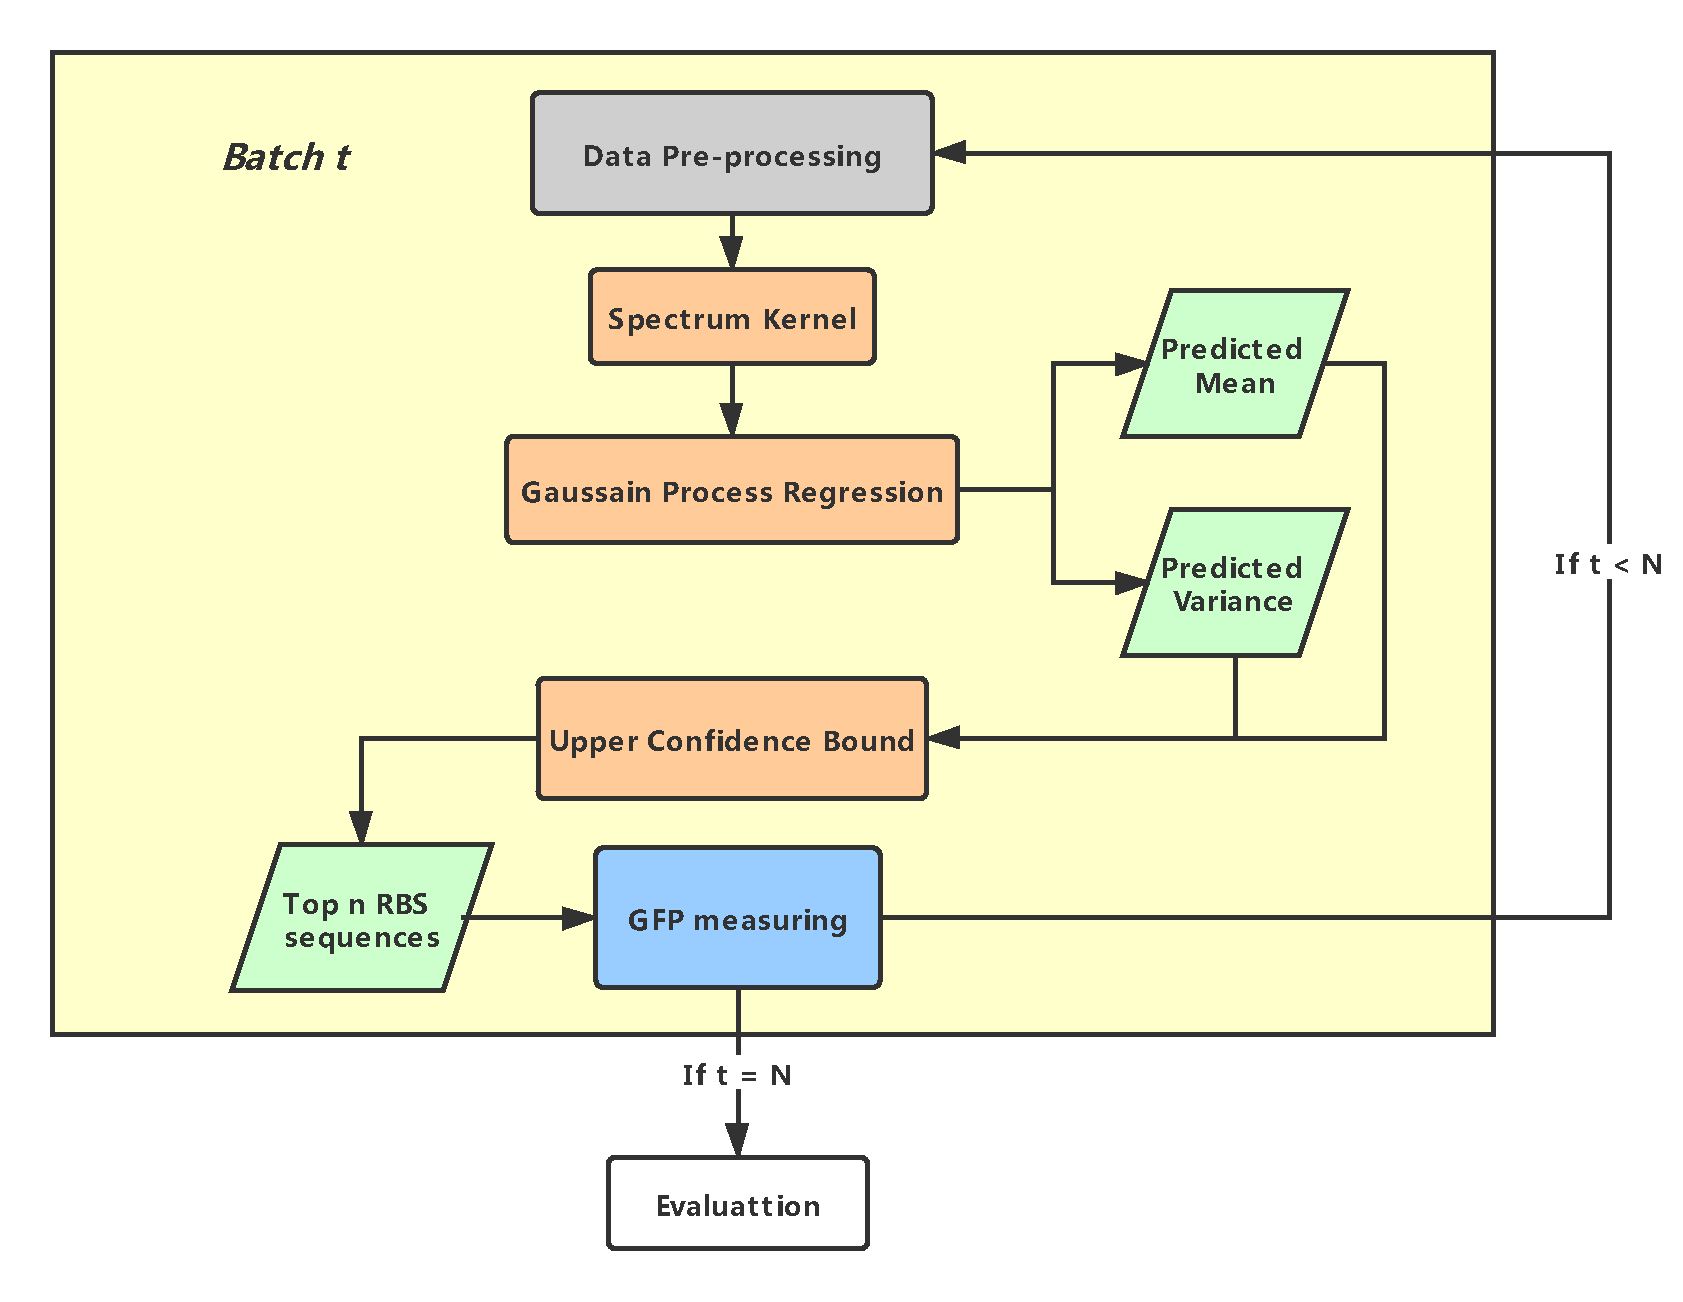
\includegraphics[scale=0.7]{plots/flowchart.pdf}
    \caption{Flowchart of machine learning based experimental design.}
    \label{fig: flowchart of machine learning based experimental design.}
\end{figure}

\subsubsection{LEARN: Gaussian Process Regression with String Kernel}

To find RBS sequences with the largest possible TIR score after a total number of rounds $N$,  we consider our experimental design problem as sequentially optimising an unknown reward function $f: \mathcal{D} \rightarrow \mathbb{R}$, where $\mathcal{D}$ is the set containing all RBS sequence points, and $f(\mathbf{x})$ is the TIR score at $\mathbf{x}$. 
In each round $t$, we choose a set of $m$ points $\mathcal{S}_t \subset \mathcal{D}$ and observe the function values of each points in the selected set $\mathcal{S}_t$, i.e. $y_i = f(\mathbf{x}_i) + \epsilon_i$, for all $i \in \mathcal{S}$, where $\epsilon_i$ is the noise (we assume the noise is following Gaussian distribution with unknown mean and variance). This noise is influenced by the accuracy of the RBS predictor and other experimental interference (e.g. time, temperature, operator, etc.). 

For regression model, we consider the \textit{Gaussian Process Regression (GPR)}.
A Gaussian process regression model \cite{Rasmussen2004} is a Bayesian approach which provides uncertainty measurements on predictions. 
We model $f$ as a sample from a \textit{Gaussian process} $\mathcal{G} \mathcal{P}(\mu(\mathbf{x}), k(\mathbf{x}, \mathbf{x'}))$, which is specified by the mean function $\mu(\mathbf{x})=\mathbb{E}[f(\mathbf{x})]$ and the kernel (or covariance) function $k\left(\mathbf{x}, \mathbf{x}^{\prime}\right)=\mathbb{E}[(f(\mathbf{x})-\left.\mu(\mathbf{x}))\left(f\left(\mathbf{x}^{\prime}\right)-\mu\left(\mathbf{x}^{\prime}\right)\right)\right]$.
%As illustrated in Figure \ref{fig: Gaussian Process Regression Example.}, 
GPR can predict both the posterior mean and posterior variance. The posterior variance represents the level of uncertainty for the prediction. 
% We assume the observations are noisy, so even when a data point in observed then confidence interval is still bigger than 0. 
% As we can see, the true function is in the confidence interval when there are data points are observed. 

% \begin{figure}[t]
%     \centering
%     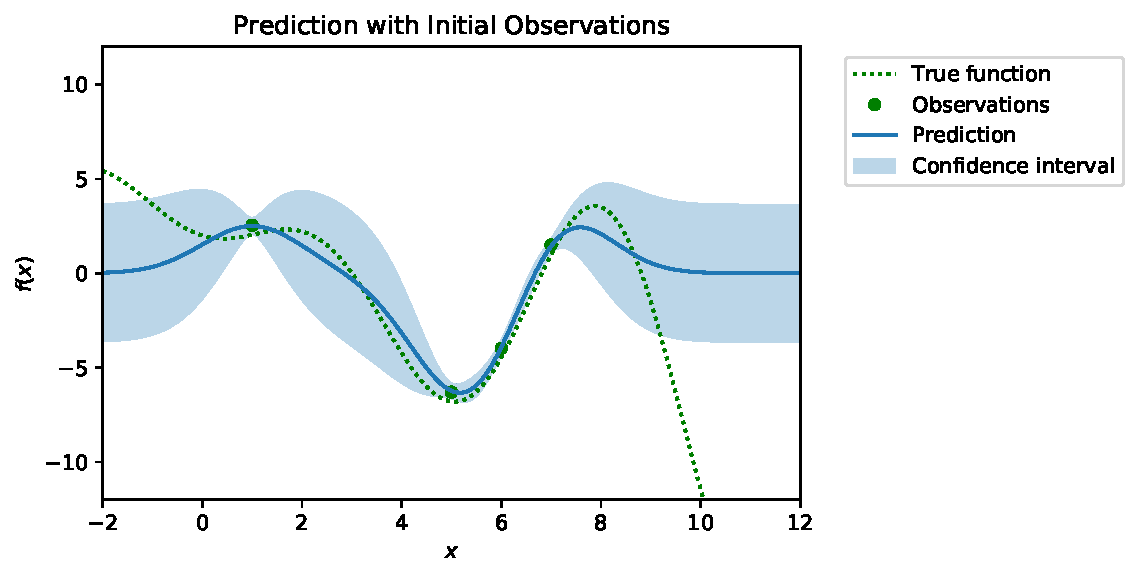
\includegraphics[scale=0.7]{plots/Prediction with Initial Observations.pdf}
%     \caption{Gaussian Process Regression Example. This plot shows the GPR prediction with confidence interval based on 4 initial observations. The confidence interval are shown in predicted mean $\pm$ 1.96 standard deviation.}
%     \label{fig: Gaussian Process Regression Example.}
% \end{figure}

The choice of covariance functions is critical for accurate predictions, which controls smoothness and amplitude of the function we model.
To represent the RBS sequences and formulate the similarity between sequences, we use the \textit{weighted degree kernel with shift} (WDS) \cite{ratsch_rase_2005} to specify the kernel function of $GP$.  
WDS is one type of string kernels, which takes two sequences as inputs and outputs a scalar value which represents the similarities between the two sequences.  
DS kernel counts the match of substrings with different length (i.e. kmers) starting for different positions. 
The WDS considers the positional information and allows positional shifts for matching substrings.
Let $\mathbf{x}, \mathbf{x}^\prime$ be two RBS sequences. 
And let $\ell$ be the maximum length of substrings taking into account, $L$ be the length of sequences, and $S(l)$ be the maximum shift length for substrings starting from position $l$.
\begin{align}
        k_\ell^{WDS}(\mathbf{x}, \mathbf{x}^\prime) 
        %&= \sum_{d=1}^{\ell} \beta_d \sum_{l=1}^{L-d+1} \gamma_l \sum_{s = 0, s + l \leq L}^{S(l)} \delta_s
        %\left(k_d^{Spec}(\mathbf{x}_{[l+s:l+s+d]}, \mathbf{x}_{[l:l+d]}^\prime) + (k_d^{Spec}(\mathbf{x}_{[l:l+d]}, \mathbf{x}_{[l+s:l+s+d]}^\prime)\right)\\
        = \sum_{d=1}^{\ell} \beta_d \sum_{l=1}^{L-d+1} \gamma_l \sum_{s = 0, s + l \leq L}^{S(l)} \delta_s
        \left(\mathbb{I}(\mathbf{x}_{[l+s:l+s+d]} = \mathbf{x}_{[l:l+d]}^\prime) + (\mathbb{I}(\mathbf{x}_{[l:l+d]}= \mathbf{x}_{[l+s:l+s+d]}^\prime)\right),
\end{align}
where 
$\beta_d = \frac{2(\ell - d + 1)}{\ell(\ell+1)}, \delta_s = \frac{1}{2(s+1)}$, $\gamma_l$ is a weighting over the position in the
sequence, where we choose to use a uniform weighting over the sequences, i.e. $\gamma_l = 1/L$. $S(l)$ determines the shift
range at position $l$. 
$\mathbb{I}$(A) is the indicator function, which equals 1 if $A$ is true and 0 otherwise. 

$\mathbb{I}(\mathbf{x}_{[l+s:l+s+d]} = \mathbf{x}_{[l:l+d]}^\prime)$ basically counts the matches of substrings of length $d$ between $\mathbf{x}$ starting from position $l+s$ and $\mathbf{x}^\prime$ starting from position $l$.
Similarly for $\mathbb{I}(\mathbf{x}_{[l:l+d]}= \mathbf{x}_{[l+s:l+s+d]}^\prime)$.
By having these two terms considering substrings of two sequences with starting positions differing $s$ characters, the WDS can measure the shifts positional information. 
When $s = 0$, the kernel function counts the matches for no shift between sequences. 
    
    
%  For recommendations, we consider the \textit{Upper Confidence Bound (UCB)} type algorithms. 
%  As one popular type of the bandit algorithms \cite{lattimore2018bandit}, the UCB type of algorithms are based on the \textit{optimism in the face of uncertainty},
 %provide various approaches to sequential design where an agent adaptively chooses one or more options among several actions based on certain policies. In our work we used the Upper Confidence Bound version of that algorithm, which is based on the \textit{optimism in the face of uncertainty}. The UCB algorithm, as the name suggests,
%  which basically select RBS sequences with the maximum upper confidence bound constructed by the sum of the predicted mean and $n$ standard deviation ($n > 0$), i.e. $\operatorname{argmax}_{\mathbf{x}_i \in \mathcal{D}} \left( \mu_t(\mathbf{x}_i) + \beta_t \sigma_t(\mathbf{x}_i)\right)$,
%     where $\beta_t$ is a hyperparameter balancing the exploitation and exploration, 
%     $\mu_t(\mathbf{x}_i), \sigma_t(\mathbf{x}_i)$ are the predicted mean and standard deviation at round $t$ for the sequence $\mathbf{x}_i$. 

\subsubsection{DESIGN: Batch UCB}

For recommending RBS sequences to label, we consider the Upper Confidence Bound (UCB) algorithm, 
%which is based on the \textit{optimism in the face of uncertainty}, 
selecting RBS sequences with the maximum upper confidence bound at round $t$, i.e.
\begin{align}
\label{Eq: GPUCB}
    \operatorname{argmax}_{\mathbf{x}_i \in \mathcal{D}} \left( \mu_{t-1}(\mathbf{x}_i) + \beta_t \sigma_{t-1}(\mathbf{x}_i)\right),
\end{align}
where $\beta_t$ is a hyperparmeter balancing the exploitation and exploration, 
$\mu_t(\mathbf{x}_i), \sigma_t(\mathbf{x}_i)$ are the predicted mean and standard deviation (SD) at round $t$ for the sequence $\mathbf{x}_i$.
We call $\mu_{t-1}(\mathbf{x}_i) + \beta_t \sigma_{t-1}(\mathbf{x}_i)$ as \textit{UCB score} of sequence $\mathbf{x}_i$ at round $t$.

Since labelling sequences is time-consuming, it is unrealistic to recommend sequence sequentially (i.e. one-by-one) and waiting for the label for each round.
Consider the task of recommending RBS sequences in a batch of size $n$. 
One naive approach is to train GPR on sequences with known TIR labels and recommend sequences in design space with top $n$ UCB scores, as shown in Figure \ref{fig: Top UCB rec.} ($n = 2$).
This approach may end up recommending similar sequences in neighbourhood (e.g. $x = 2, x =2.5$ in this example). 
However, since we assume similar sequences would have similar labels (e.g. by knowing $x=2$ we can gain information of $x=2.5$ as well), we prefer to not waste time and money on labelling sequences with high similarities in a batch.

\begin{figure}[t]
    \centering
    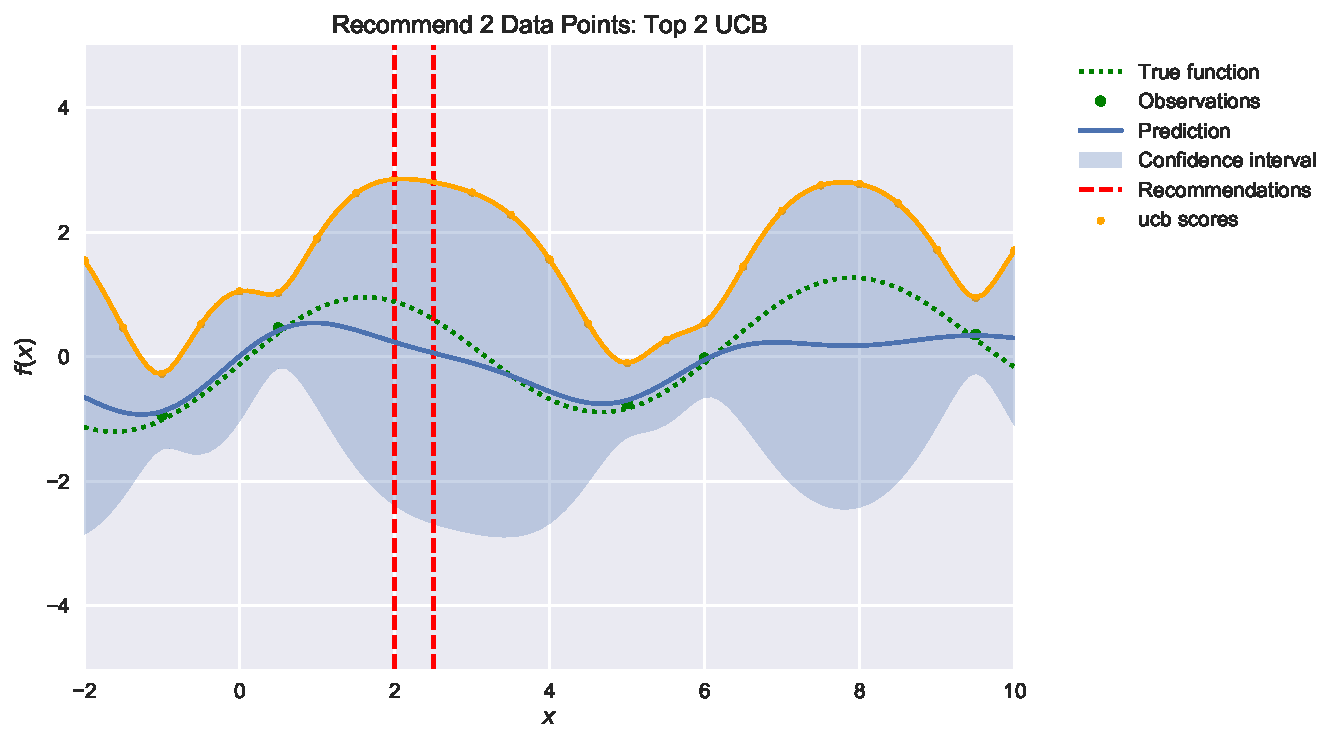
\includegraphics[scale=0.6]{plots/Recommend_2_Data_Points:_Top_2_UCB.pdf}
    \caption{Batch Recommendation: Top UCB scores. We consider the batch size 2, with 5 initial observations. The design (recommendation) space is 24 uniformly distributed points in the range [-2,10], i.e. {-2, -1.5, -1, ..., 9.5, 10}. The recommendations are 2 data points with top UCB scores, constructed with GPR predictions. The confidence interval are shown in predicted mean $\pm$ 1.96 standard deviation. }
    \label{fig: Top UCB rec.}
\end{figure}

A key property of Gaussian Process regression is that the predictive variance only depends on observed points (i.e. features), but not on the labels of those observed points. 
% We illustrate this fact by comparing the prediction with the true function value of the new recommended point (Figure \ref{fig: Recommend 1 Data Point (New Observation)}) and the prediction with the predicted value of the new recommended point (Figure \ref{fig: Recommend 1 Data Point (Predicted Mean)}).
% As we can see, the predicted confidence interval is the same for the two plots. 
We can make use of this property to design batch upper confidence bound (BUCB) algorithm \cite{desautels2012parallelizing}.
That is, recommend sequences sequentially by assuming have seen the previous recommended points and updating the UCB score with the updated predicted SD. 
% Figure \ref{fig: Recommend 2 Data Points: GP-BUCB.} shows an example of batch UCB recommendation. 
% The plot shows the predicted mean and variance after observing 4 data points. 
Consider the same setting in Figure \ref{fig: Top UCB rec.} as an toy example, GP-BUCB firstly recommend the data point with maximum UCB scores based on the predictions over initial 5 observations. 
As shown in Figure \ref{fig: GP-BUCB:_Recommend_1st_Data_Point.}.  
Then we add the recommended data point ($x = 2$) into training data with the predicted mean of that point as label (note it is not the true label, i.e. observation), and update the predicted variance then update the UCB scores. 
We recommend the second data point based on the new UCB scores.   
As we can see, since we assume we have observed $x = 2$, then the new predicted variance of the data points in design space around $x =2$  decreases, so instead of recommending a similar data point $x = 2.5$, we recommend the data point which is in another area and potentially having high labels ($x = 7.5$).     
By using GP-BUCB, we rule out the sequences with high similarities in the same batch and increase the exploration efficiency. 
2 data points ($x = 8, x = 0$) are recommended in batch. 

\vspace{0.5cm}
\begin{minipage}{\textwidth}
  \begin{minipage}[b]{0.49\textwidth}
    \centering
    %\includegraphics[scale=0.4]{plots/Hist.pdf}
    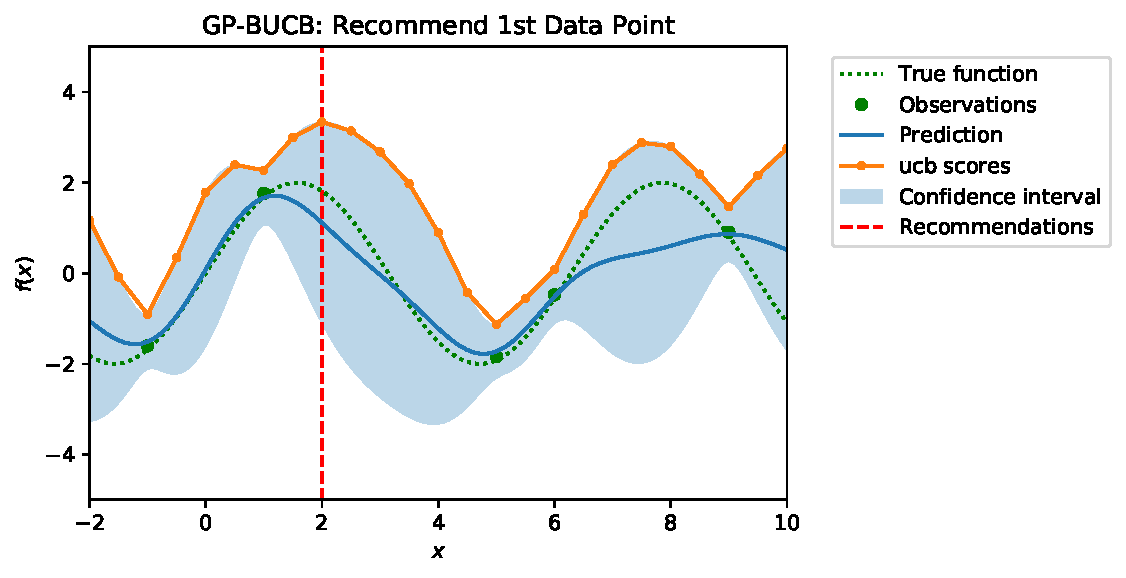
\includegraphics[scale=0.45]{plots/GP-BUCB:_Recommend_1st_Data_Point.pdf}
     \captionsetup{type=figure}
     \vspace{-0.5cm}
    \caption{GP-BUCB: Recommend 1st Data Point.}
    \label{fig: GP-BUCB:_Recommend_1st_Data_Point.}
\end{minipage}
  \hfill
  \begin{minipage}[b]{0.49\textwidth}
    \centering
    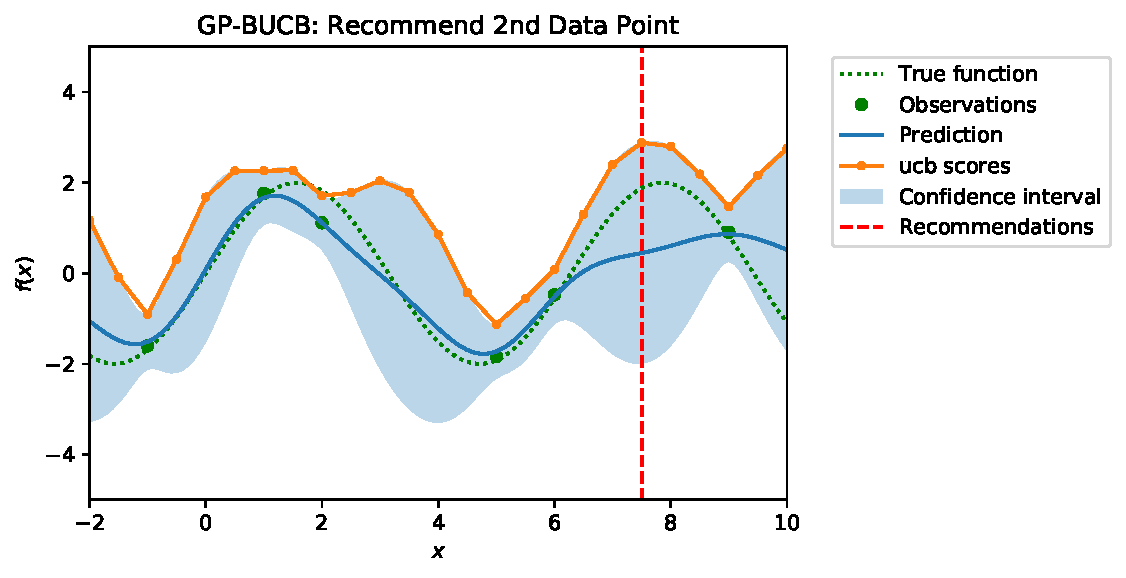
\includegraphics[scale=0.45]{plots/GP-BUCB:_Recommend_2nd_Data_Point.pdf}
     \captionsetup{type=figure}
     \vspace{-0.5cm}
    \caption{GP-BUCB: Recommend 2nd Data Point.
    }
    \label{fig: GP-BUCB:_Recommend_2nd_Data_Point.}
 \end{minipage}
 \end{minipage}
 \vspace{0.5cm}







